%%%%%%%%%%%%%%%%%%%%%%%%%%%%%%%%%%%%%%%%%%%%%%%%%%%%%%%%%
%          File: CascadedTunableFilter.tex            	%
%                  Date: 2 Feb, 2015                	%
%                                                    	%
%   For submission to a journal  						%
%                                                     	%
%   Technical paper about the results obtained with   	%
%   professor Wei Shi with tunable cascaded				%
%	contra-directional coupler				      		%
%	+ theorical analysis								%
%%%%%%%%%%%%%%%%%%%%%%%%%%%%%%%%%%%%%%%%%%%%%%%%%%%%%%%%%

\documentclass[9pt,twocolumn,twoside]{osajnl}

\journal{ol} % Choose journal (ao, josaa, josab, ol)

\setboolean{shortarticle}{true}

\usepackage{ulem}
\usepackage{amsmath,amssymb}
\newcommand{\me}{\mathrm{e}}
\newcommand*\diff{\mathop{}\!\mathrm{d}}



\usepackage{graphicx,epsfig,epstopdf}



\title{Ultra-compact, widely bandwidth-tunable filter using cascaded silicon photonic contra-directional couplers}



\author[1]{Jonathan St-Yves}
\author[1]{Hadi Bahrami}
\author[1]{Philippe Jean}
\author[1]{Sophie Larochelle}
\author[1,*]{Wei Shi}
\affil[1]{Centre d'optique, photonique et laser (COPL) and Département de génie électrique et génie informatique, Université Laval, 2375 rue de la Terrasse, Québec (Québec), Canada, G1V 0A6}
\affil[*]{Corresponding author: wei.shi@gel.ulaval.ca}

\dates{Compiled \today}

\ociscodes{ (130.7408) Wavelength filtering devices; (350.2770) Gratings; (130.3120)   Integrated optics devices}

\doi{\url{http://dx.doi.org/10.1364/ao.XX.XXXXXX}}

\begin{abstract}
We demonstrate an integrated tunable band-pass filter continuously tuned from 788 GHz down to 117 GHz of bandwidth with up to 3 nm of central wavelength tunability in the infrared C-band. The out-of-band contrast is up to 55 dB, the in-band ripples are under 0.3 dB and the free spectral range is unlimited. This result was achieved using contra-directional couplers and micro-heaters on the silicon-on-insulator platform with a footprint of less than 0.007 mm$^2$. An other iteration pushing the tunability from 1 THz to 100 GHz is discussed. 
\end{abstract}


\setboolean{displaycopyright}{true}

\begin{document}
\maketitle
\thispagestyle{fancy}
\ifthenelse{\boolean{shortarticle}}{\abscontent}{}

%\section{Introduction}

Next-generation optical transmission systems applying flexible networking and the super-channel technique will require highly dynamic channel allocation to drastically increase the spectral efficiency and transmission capacity \cite{jinno2009spectrum, geisler2011demonstration}.
Tunable optical filters, reconfigurable in both center wavelength and bandwidth with scalability towards terahertz \cite{geisler2011demonstration}, are essential for these applications.
Such large bandwidth tunability is currently only available in bulky bench-top systems using diffractive grating spectrometers or liquid crystals.
Integrated solutions are desired for lower cost and power consumption.
In particular, silicon photonics  based on the sub-micron silicon-on-insulator platform allows for CMOS compatible mass fabrication, enabling low cost, high yield, and high-density chip-scale integration.
Existing solutions for tunable  filters on silicon include devices based on microring resonators \cite{DynamicBW, ong2013ultra} and Mach-Zehnder interferometers (MZIs). These devices have relatively small tunable bandwidth (less than 200 GHz) and small free spectral range (FSR) (typically less than 10 nm), not suitable for high-capacity transmission applications.

Contra-directional couplers(contra-DCs) are grating-assisted add-drop filters \cite{shi2013siliconContraDC}. 
Analogous to waveguide Bragg gratings, the wavelength selectivity in contra-DCs is based on periodic dielectric perturbations. But instead of back-reflections in the same waveguide, the selected wavelength in a contra-DC is dropped to another waveguide through contra-directional coupling.
This allows add-drop operation without the need of a circulator. 
Contra-DCs have merits of compactness, flat-top response, flexible filter design (e.g, through apodization), and near-infinite FSR (in the case of first-order gratings).
In particular, they allow for very high bandwidths (greater than 10 nm) and thus can support very-high-baud-rate super-channel signals \cite{jinno2009spectrum}.
In this paper, we demonstrate a broadband filter with a large tunability in both wavelength and channel bandwidth, using thermally controlled cascaded contra-DCs on a silicon chip. 
The filter has flat-top responses, low insertion loss, low in-band ripples, and high contrast between the pass-band and the stop-band.

\begin{figure}[htbp]
	\centering
	\includegraphics[width=1.00\columnwidth]{data/CascadedSchematic2}
	\centering
	\caption{Schematic of the device. 
	The dropped wavelength of the first contra-directional coupler is re-filtered in an identical component. 
	Both contra-directional couplers are temperature-controlled with metal heaters. 
	Plots show examples of spectrum at each port, on a logarithmic scale.}
	\label{fig:schematic}
\end{figure}
%\section{Principle and Design}

The schematic of the proposed device is shown in Fig.~\ref{fig:schematic}. 
It consists of a pair of cascaded contra-DCs, each operating as a drop filter. 
The drop port of the first contra-DC is connected to the input port of the second contra-DC. 
Therefore, the finally dropped signal is determined by the product of the  drop-port transfer functions of the two contra-DCs. 

The center wavelength of a contra-DC is determined by the phase-match condition: $\lambda_\text{c} = \Lambda (n_\text{1}+n_\text{2})$, where $\lambda_\text{c}$ is the center wavelength of contra-directional coupling, $\Lambda$ is the grating pitch, and $n_\text{1}$ and $n_\text{2}$ are the effective refractive indices of the first-order and second-order eigenmodes in the coupler. 
At first, the two filters are identical and drop a large well defined window. By changing the temperature of a single filter, the bandwidth of the finally dropped signal can be adjusted by detuning their central wavelengths.



\begin{figure}[htbp]
  \centering
  \includegraphics[width=1\columnwidth]{data/FigApod}
  \caption{(a)SEM photography of a part of the grating. The contra-directional coupler consists of two close waveguides of different width with periodic sidewall corrugations. (b) Apodization profile of the grating. A larger coupling requires larger corrugations. (c) Intensity distributions of electrical fields of the first and second transverse modes. }
  \label{fig:SEM}
\end{figure} 


A broadband filter design for a coarse WDM on the 220-nm SOI platform \cite{shi2013siliconCWDM} is adopted for individual contra-DCs.  
In each contra-DC, the widths of the waveguides are of 560 and 440 nm.
This high asymmetry ensures a negligible forward cross-coupling. 
The gratings are formed by sidewall corrugations in strip waveguides with a pitch of 312 nm. 
The spacing between the waveguides varies between 65 and 135 nm to produce a Gaussian coupling profile apodization as shown in Fig.~\ref{fig:SEM} for efficient sidelobe suppression, for which details can be found in \cite{shi2013siliconCWDM}.

The spectral responses of each contra-DC is calculated using coupled mode theory, following the same procedure as in  \cite{shi2013siliconContraDC}, with three additions: apodization, temperature and noise simulation.

While an unapodized (uniform) grating can be simulated with only two transfer matrices , $S_1$ and $S_2$ \cite{shi2013siliconContraDC}, an apodized one needs both of these matrices for each step along the propagation, to match the change of coupling. 
The first change is thus to modify the transfer matrix of the system to the product of all the grating elements along the propagation axis.
Our simulations use 100 segments to approximate the constantly changing coupling.

On top of each contra-DC sits a metal strip acting as a micro-heater for thermal tuning.  
The refractive index of silicon has a temperature dependence of $\frac{\diff{n_\text{Si}}}{\diff{T}}=$ 1.87$\times10^{-4}$K$^{-1}$ at room temperature for wavelengths around 1550 nm~\cite{frey2006temperature}.
Without electrical input, the optical responses of the two filters are identical (neglecting fabrication uniformness) resulting in a sharp transition from the pass-band to the stop-band. 
Applying independent electrical currents on the heaters, we can shift the spectra of the contra-DCs simultaneously or differentially for wavelength or bandwidth tuning.
Ideally, each contra-DC should be uniformly heated so that the apodization profile isn't disturbed as the temperature varies.

In simulation, the temperature dependence is accounted for by increasing the effective index according to 
$\diff{n_\text{eff}}=\frac{\diff{n_\text{Si}}}{\diff{T}}*\frac{\diff{n_\text{eff}}}{\diff{n_\text{Si}}}*\diff{T}$, where $\frac{\diff{n_\text{eff}}}{\diff{n_\text{Si}}}$ is evaluated using an eigenmode solver.

While only coupling apodization has been discussed so far, it is common in Bragg grating profiles to also adjust the local Bragg wavelength. This is done with a phase shift changing the local effective index or period. This design only uses coupling apodization in principle, but phase noise also appears during fabrication due to non-uniformity and sidewall roughness.

There are 2 main types of waveguide noise. High frequency roughness(typically around 10 $\mu$m of spacial period\cite{simard2013characterization}) is caused by sidewall roughness and decreases the sidelobe suppression. Low frequency variation(larger than the device or 300 $\mu$m) is caused by wafer thickness and etching variance and causes a linear chirp that increases the bandwidth.

High frequency phase noise is added to the transfer matrix solution by adding random noise to the $\Delta\hat{\beta}$ propagation constants. The frequency distribution of the noise will thus match the quantization steps of the matrices, but since the response noise is dependent of both the amplitude and frequency of the sidewall roughness \cite{simard2011impact},we can fit the simulation to the experiment by choosing the right noise amplitude.
Similarly, we can also add a variation to $\Delta\hat{\beta}$ which is dependent on the longitudinal position.


%\section{Experiment}

The device was fabricated using a CMOS-compatible technology with electron-beam lithography. 
Fiber grating couplers\cite{zhong2014focusingFGC} were used as optical IOs in the measurement. 
Fig.~\ref{fig:passive} shows the measured drop port response of the cascaded contra-DC filters. 
The measurements were normalized using the response of a pair of directly connected fiber grating couplers on the same chip.
\begin{figure}[htbp]
\centering
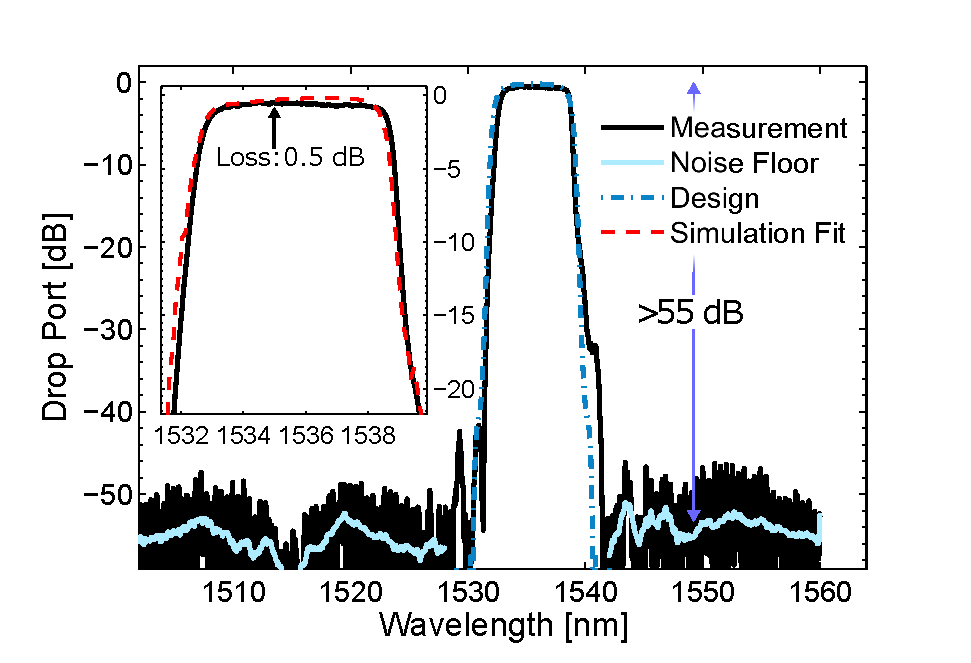
\includegraphics[width=.99\columnwidth]{data/Passive62}
\caption{ Spectral response of the cascaded filters without heating: 1-dB BW is 733 GHz, 3-dB BW is 788 GHz, 10-dB BW is 868 GHz, and 20-dB BW is 990 GHz. Inset shows the filter shape up to -20 dB, which is the typical communication requirement.}
\label{fig:passive}
\end{figure}

The device exhibits a high side-lobe suppression ratio (SLSR) of over 40 dB and a high contrast of about 55 dB between the pass-band and the stop-band. 
The insertion loss is very low, less than 0.5 dB (i.e., 0.25 dB per contra-DC), with small ripples of less than 0.3 dB within the 1-dB passband over 5.8 nm (733~GHz). 
The edge roll-off rate is 19 dB/nm on the left side and 24 dB/nm on the right side.
Further work could optimize the grating structure using the inverse layer peeling algorithm\cite{skaar2001synthesis} since the mathematics of the contra-directional coupler are similar to those of Bragg gratings.

By changing the temperature of a single contra-DC, we offset the phase-match condition of a filter, resulting in a smaller band overlap between the two contra-DCs and thus a narrower passband in the drop port, as shown in Fig.~\ref{fig:bandTune}.  
Due to the wavelength detuning,  the stop-band edges are only determined by the single filters. 
As a result, the side-lobes suppression degrades  for small bandwidths but is still better than 15 dB. A continuous tuning of the 3-dB bandwidth from 788 GHz down to 117 GHz (i.e., over 670 GHz or 5.4 nm) is experimentally observed as the on-chip temperature increases by 70 degrees. 
The smallest bandwidth measured in this case was limited by the maximal power delivered before the metal heaters (300-nm-thick, 2-$\mu$m-wide Al strips) were damaged. 
The power efficiency of the bandwidth tuning is about 24 mW/nm, which can significantly improved by optimizing the heater design, e.g., using smaller heater features and thermal isolation \cite{dong2010thermally}.

We observe that the central wavelength at higher temperature is out of the original band, indicating thermal coupling between the two filters. Also, the side-lobes suppression ratio is lower for smaller bandwidth due to the signal only being affected by one filter. To solve both of these problems, next generation devices should use a isolation or larger spacing between filter elements (we used 12 \text{$\mu$}m center to center).

\begin{figure}[htbp]
\centering
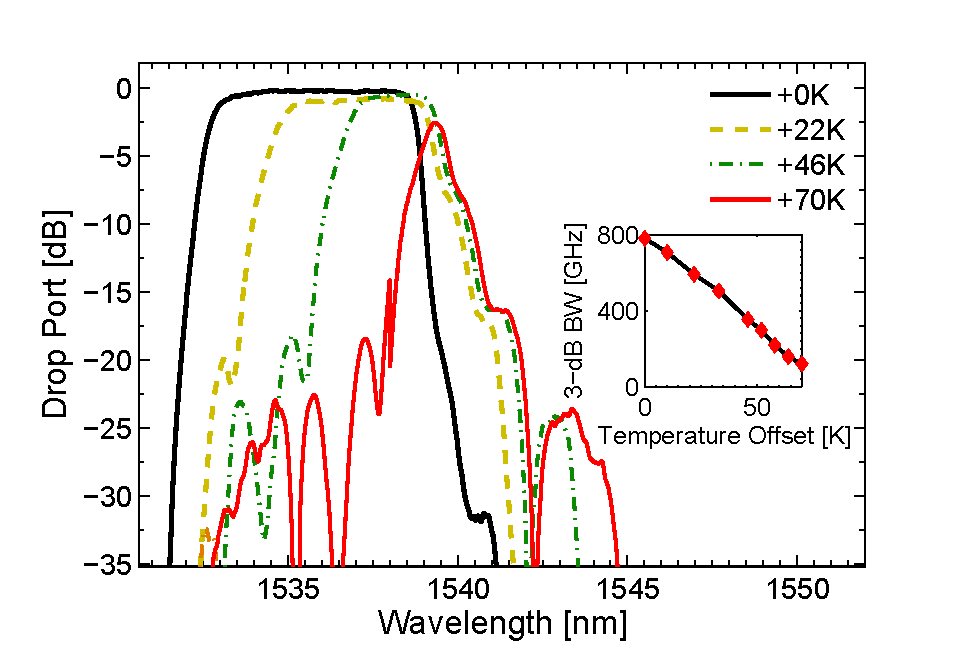
\includegraphics[width=.99\columnwidth]{data/Band6}
\caption{Spectral response of the device for different temperatures applied to only one contra-DC: 1-dB BW tuned down to 65 GHz, 3-dB BW to 117 GHz. The temperatures are obtained from simulation fit. Inset shows the temperature dependence.}
\label{fig:bandTune}
\end{figure} 
An improvement upon this design is simulated in Fig.~\ref{fig:bandTuneSimu}. By using 4 filtering elements instead of 2, and improving the thermal performances to achieve a stable high temperature, it would be possible to tune the bandwidth from over 1 THz down to under 100 GHz while still maintaining a very high out of band contrast of over 20 dB. This simulation uses the noise parameters observed in the 2 stage experiment.
\begin{figure}[htbp]
\centering
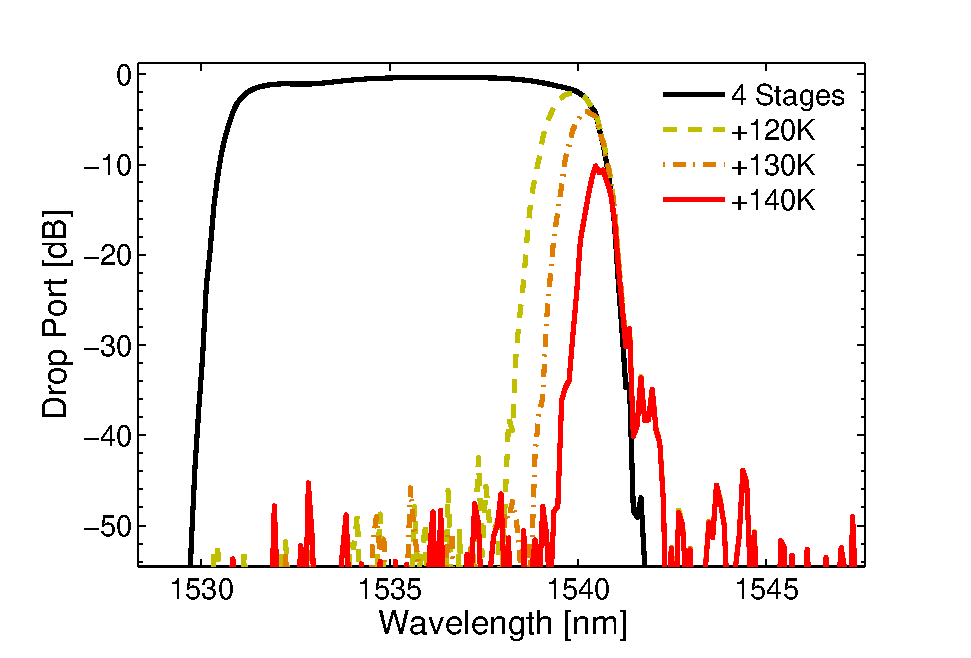
\includegraphics[width=.99\columnwidth]{data/4StageDesignCompiled}
\caption{Simulation of the spectral response with the heat applied to two out of four cascaded contra-DCs: the bandwidth can be continuously tuned from 1020 GHz to  51GHz.}
\label{fig:bandTuneSimu}
\end{figure} 

By applying the same temperature variation on both contra-DCs, the center wavelength can be tuned without affecting the filter shape.
As shown in Fig.~\ref{fig:wavTune}, when the center wavelength is continually changed over 4 nm by varying the on-chip temperature, the filter shape is maintained with sharp edges. Actually, slight detuning between the cascaded contra-DCs may be used to compensate for band-edge distortions due to fabrication errors for a more symmetric filter shape. 
The power efficiency of the wavelength tuning is about 44 mW/nm, which is about twice the power consumption of the bandwidth tuning since two contra-DCs are heated simultaneously.
\begin{figure}[htbp]
\centering
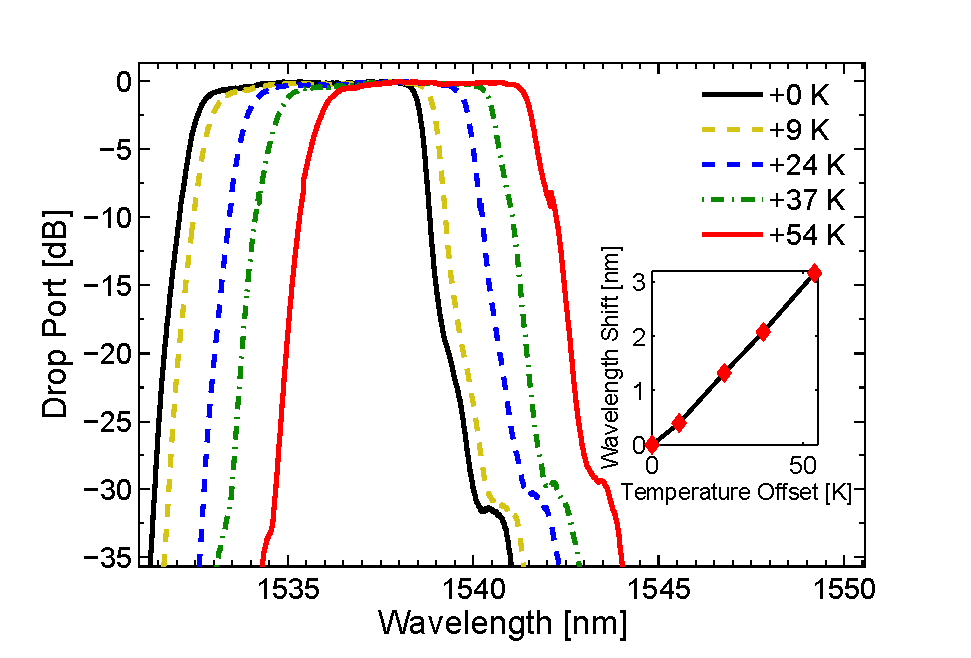
\includegraphics[width=.99\columnwidth]{data/Central2}
\caption{Spectral response with the heat applied to both contra-DCs: the central wavelength is tuned from 1535 nm to 1539 nm continuously; the temperatures are calculated by comparison to simulation. Inset shows the temperature dependence.}
\label{fig:wavTune}
\end{figure} 




%\subsection{Phase/dispertion}
An other important parameter to monitor is the group delay of the device. An uneven delay can cause distortion during detection of the signal, just like dispersion. The simulation and measurements seen in Fig.~\ref{fig:phase} both show a group delay difference of less than 10 ps.
\begin{figure}[tbp]
\centering
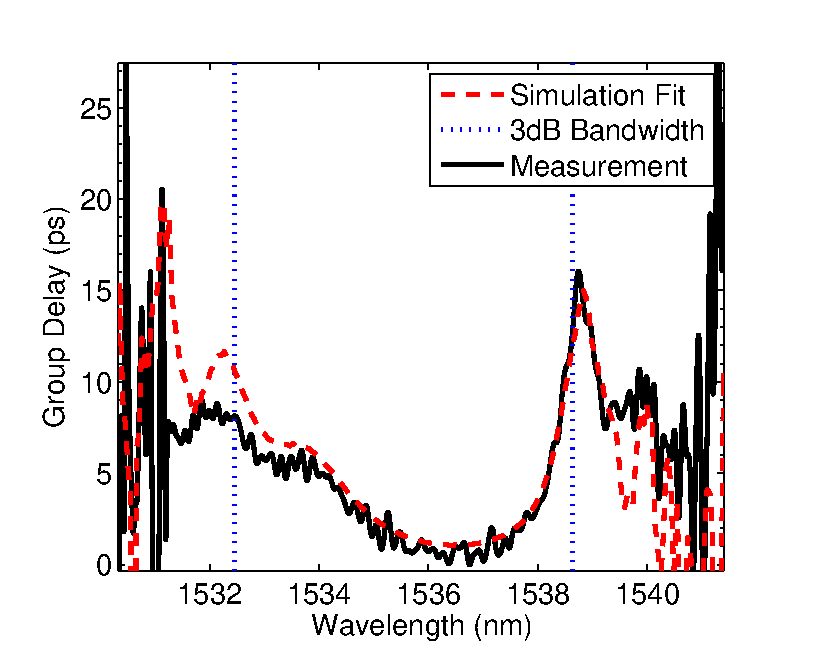
\includegraphics[width=.99\columnwidth]{data/Phase2}
\caption{ Group delay response of the tunable filter at the drop port. The delay stays within 12 ps between any two points in the band. The out of band results are noisy due to the weak signal.}
\label{fig:phase}
\end{figure}

Table \ref{table:comparison} shows a comparison of this filter with other recent publications of tunable filters. No other tunable filter has such a large available bandwidth and FSR, making contra-DC unique in their application potential.


%\section{Conclusion}
In summary, we have demonstrated a bandwidth tunable filter with a low insertion loss of less than 0.5 dB, low ripples of less than 0.3 dB, a large maximal bandwidth of greater than 750 GHz, and high contrast of 55 dB. 
A large bandwidth tuning range over 670 GHz has been achieved, which, to the best of our knowledge, is the widest ever demonstrated on a silicon chip. 
This ultra-wide bandwidth tunability makes the device very attractive for next-generation ultrahigh baud-rate applications (e.g., high-capacity super-channel transmissions) and flexible optical networking. 


\begin{table*}[thb]
\caption{Recent results with multi-element on-chip silicon filters}
\begin{tabular}{cccccc}
    \hline
	Publication & Filter type & BWmax / FSR & Tunable BW & On-chip loss & Contrast \\
    \hline
    %Ibrahim (2011) &	Cascaded MRs &	0.4 GHz / 10 GHz &	0.6-2 GHz &	0.6 dB &	30 dB
    % \\
    %Alipour (2011) &	Cascaded MRs &	5 GHz / 650 Ghz &	0.8-5 GHz &	1.25-3.75 dB &	38 dB
    % \\
    Ding (2011)\cite{ding2011bandwidth} &	MRs + MZI &	55 GHz / 1 THz &	28-55 GHz &	3.6 dB &	30 dB
     \\
 	Orlandi (2012)\cite{orlandi2012reconfigurable} &	MRs + MZI &	173 GHz / 200 GHz &	23-173 GHz &	0.46-1.06 dB &	15-34 dB
      \\
    %Luo (2012) &	Cascaded MRs &	100 GHz / 750 Ghz &	No &	0.3-0.6 dB &	50 dB  \\
    Ong (2013)\cite{ong2013ultra} &	Cascaded MRs &	125 GHz/ 0.9 THz &	11.6-125 GHz &	0.25 dB &	50-100 dB
      \\
    \textbf{This experiment }& Cascaded contra-DC &	778 GHz / Unlimited  &	117-778 GHz &	0.5 dB &	55 dB 
    \\
    \textbf{4 Stages }& Cascaded contra-DC &	1020 GHz / Unlimited  &	51-1020 GHz &	<1 dB &	>55 dB 
    \\
    
    \hline
    \label{table:comparison}
   \end{tabular}
    \end{table*}




\section*{Acknowledgments}
We acknowledge CMC Microsystems for the  software and the fabrication subsidy. We thank Yun Wang and Lukas Chrostowski with the Univeristy of British Columbia for the fiber grating coupler design. The authors acknowledge the Natural Sciences and Engineering Research Council of Canada, TeraXion and Prompt for funding this research. The silicon chip was fabricated at the University of Washington Microfabrication/Nanotechnology User Facility, a member of the NSF National Nanotechnology Infrastructure Network.


\bibliography{bibli}

\end{document}